%Correct the file name.
%X: book number
%Y: part number
%ZZZ: page number in three digits. So page 3 would be 003.

\documentclass[11pt]{amsbook}

\usepackage{../HBSuerDemir}	% ------------------------


\begin{document}

% ++++++++++++++++++++++++++++++++++++++
\hPage{b2p1/11}
% ++++++++++++++++++++++++++++++++++++++

\begin{center}
$\lvert a_n - a \rvert < \varepsilon$, $\lvert b_n - b \rvert < \varepsilon$ for all $n>N$
\end{center}

To show $\lvert a_n - a \rvert < \varepsilon$ we from $a_n b_n - ab$ and get

\begin{flalign*}
	\lvert a_n b_n - ab \rvert &= \lvert a_n b_n - ab_n - ab + ab_n \rvert \\
	&= \lvert (a_n - a)b_n - a(b - b_n) \rvert \\
	&\leqslant \lvert a_n - a \rvert \lvert b_n \rvert + \lvert a \rvert \lvert b - b_n \rvert \\
	&\leqslant \lvert b_n \rvert \varepsilon + \lvert a \rvert \varepsilon
\end{flalign*}

Since for all $n>N$, $b_n$ lies in the interval ($b-\varepsilon$, $b-\varepsilon$) it follows that $b_n < K$ for some positive $K$, and one has

\begin{equation*}
	\lvert a_n b_n - ab \rvert < K \varepsilon + \lvert a \rvert \varepsilon = (K + \lvert a \rvert) \varepsilon
\end{equation*}

\noindent showing that $a_n b_n \rightarrow ab$. \\

\textbf{Theorem 2}
\begin{enumerate}[label={\alph*)}]
	\item A monotone sequence is convergent,
	\item A convergent sequence is bounded,
	\item $(a_n) \rightarrow a$, $(b_n) \rightarrow n$ and $a_n \leqslant c_n \leqslant b_n$ for all $n>N \implies (c_n) \rightarrow c$ and $a \leqslant c \leqslant b$
\end{enumerate}

\textbf{Proof.} Omitted

% =======================================================
\end{document}  

%==== templates ====

%==== environments ====

%\begin{figure}[htb]
%	\centering
%	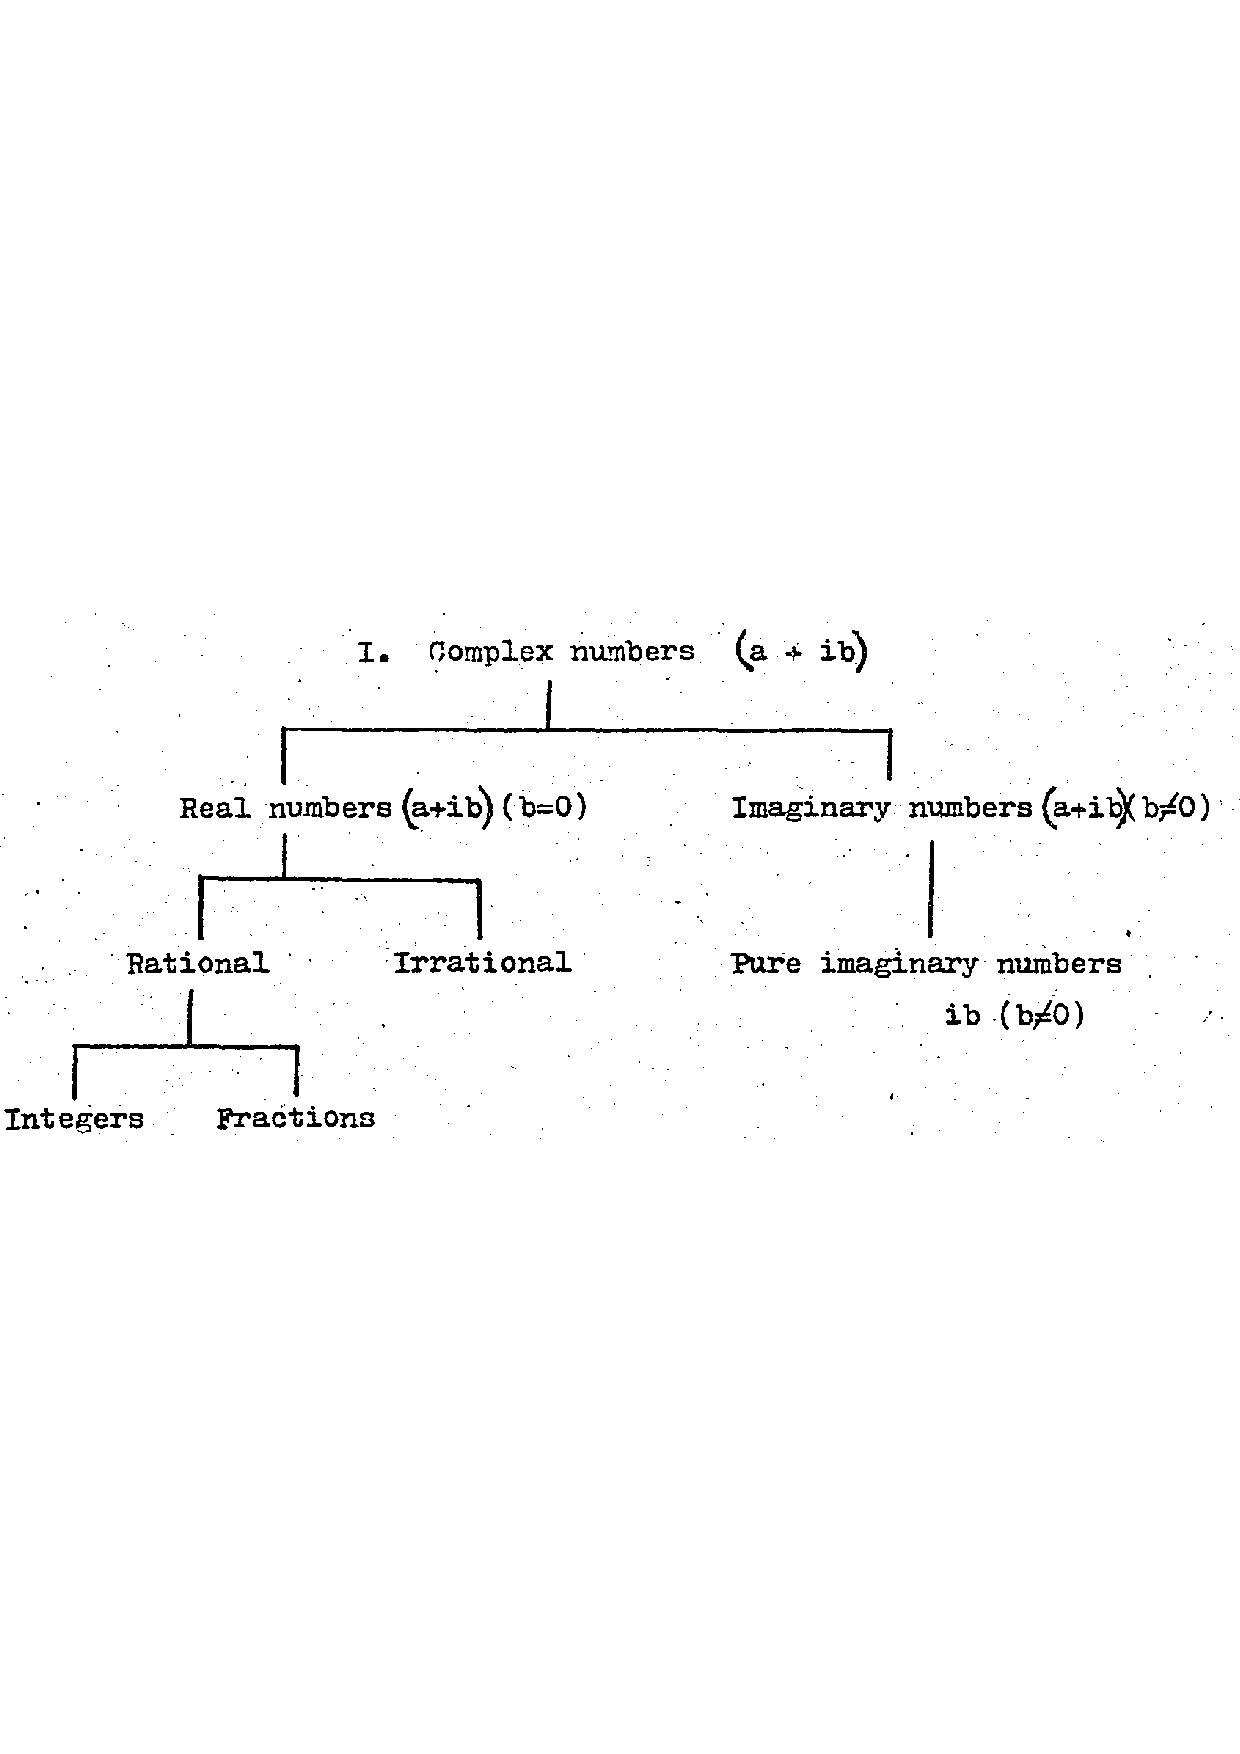
\includegraphics[width=0.9\textwidth]{images/SD-1-1p15A}
%	\caption{Classification of complex numbers}
%	\label{fig:classificationOfComplexNumbersA}
%\end{figure}

%\begin{center}
%\begin{tabular}{cc}
%\end{tabular}
%\end{center}

%\begin{exmp}
%\begin{hSolution}
%\end{hSolution}
%\end{exmp}

%\begin{hEnumerateAlpha}
%\end{hEnumerateAlpha}

%\begin{hEnumerateRoman}
%\end{hEnumerateRoman}

%$
%\begin{bmatrix}
%\end{bmatrix}
%$

%\frac{aaaa}{bbb}
%\frac{a_{n}}{b_{n}}
%\left( aaaa \right)
%\Longrightarrow

%\begin{multicols}{2}
%	bb
%\columnbreak
%	aa
%\end{multicols}
